\documentclass[]{article}
\usepackage{lmodern}
\usepackage{amssymb,amsmath}
\usepackage{ifxetex,ifluatex}
\usepackage{fixltx2e} % provides \textsubscript
\ifnum 0\ifxetex 1\fi\ifluatex 1\fi=0 % if pdftex
  \usepackage[T1]{fontenc}
  \usepackage[utf8]{inputenc}
\else % if luatex or xelatex
  \ifxetex
    \usepackage{mathspec}
  \else
    \usepackage{fontspec}
  \fi
  \defaultfontfeatures{Ligatures=TeX,Scale=MatchLowercase}
\fi
% use upquote if available, for straight quotes in verbatim environments
\IfFileExists{upquote.sty}{\usepackage{upquote}}{}
% use microtype if available
\IfFileExists{microtype.sty}{%
\usepackage{microtype}
\UseMicrotypeSet[protrusion]{basicmath} % disable protrusion for tt fonts
}{}
\usepackage[margin=1in]{geometry}
\usepackage{hyperref}
\hypersetup{unicode=true,
            pdfborder={0 0 0},
            breaklinks=true}
\urlstyle{same}  % don't use monospace font for urls
\usepackage{graphicx,grffile}
\makeatletter
\def\maxwidth{\ifdim\Gin@nat@width>\linewidth\linewidth\else\Gin@nat@width\fi}
\def\maxheight{\ifdim\Gin@nat@height>\textheight\textheight\else\Gin@nat@height\fi}
\makeatother
% Scale images if necessary, so that they will not overflow the page
% margins by default, and it is still possible to overwrite the defaults
% using explicit options in \includegraphics[width, height, ...]{}
\setkeys{Gin}{width=\maxwidth,height=\maxheight,keepaspectratio}
\IfFileExists{parskip.sty}{%
\usepackage{parskip}
}{% else
\setlength{\parindent}{0pt}
\setlength{\parskip}{6pt plus 2pt minus 1pt}
}
\setlength{\emergencystretch}{3em}  % prevent overfull lines
\providecommand{\tightlist}{%
  \setlength{\itemsep}{0pt}\setlength{\parskip}{0pt}}
\setcounter{secnumdepth}{0}
% Redefines (sub)paragraphs to behave more like sections
\ifx\paragraph\undefined\else
\let\oldparagraph\paragraph
\renewcommand{\paragraph}[1]{\oldparagraph{#1}\mbox{}}
\fi
\ifx\subparagraph\undefined\else
\let\oldsubparagraph\subparagraph
\renewcommand{\subparagraph}[1]{\oldsubparagraph{#1}\mbox{}}
\fi

%%% Use protect on footnotes to avoid problems with footnotes in titles
\let\rmarkdownfootnote\footnote%
\def\footnote{\protect\rmarkdownfootnote}

%%% Change title format to be more compact
\usepackage{titling}

% Create subtitle command for use in maketitle
\newcommand{\subtitle}[1]{
  \posttitle{
    \begin{center}\large#1\end{center}
    }
}

\setlength{\droptitle}{-2em}

  \title{}
    \pretitle{\vspace{\droptitle}}
  \posttitle{}
    \author{}
    \preauthor{}\postauthor{}
    \date{}
    \predate{}\postdate{}
  

\begin{document}

\subsection{Klassifikation}\label{klassifikation}

Durch die Wortklassifizierung konnten 2726 Anfragen eindeutig
klassifiziert werden. Weitere 253 Anfragen konnten durch die
Wortklassifizierung zu 2 oder 3 Themen zugeordnet werden. Diese Anfragen
wurden manuell richtig klassifiziert. Darüber hinaus wurden die
Anfragen, welche durch die Wortklassifizierung nur einem Thema
zugeordnet werden konnten, überprüft und bei wenigen Fällen korrigiert.
Anschließend wurden weitere wenige Anfragen manuell kategorisiert um die
Datengrundlage für die nachfolgenden Schritte der Kategorisierung weiter
vergößern zu können. Auf diese Weise wurden 3047 der insgesamt 6349
Anfragen kategorisiert. In Abbildung \ref{word_classification} ist die
Verteilung der Themen ersichtlich.

\begin{figure}[!h]
    \caption{Verteilung der Themen nach Wortklassifikation}
    \label{word_classification}
    \centering
    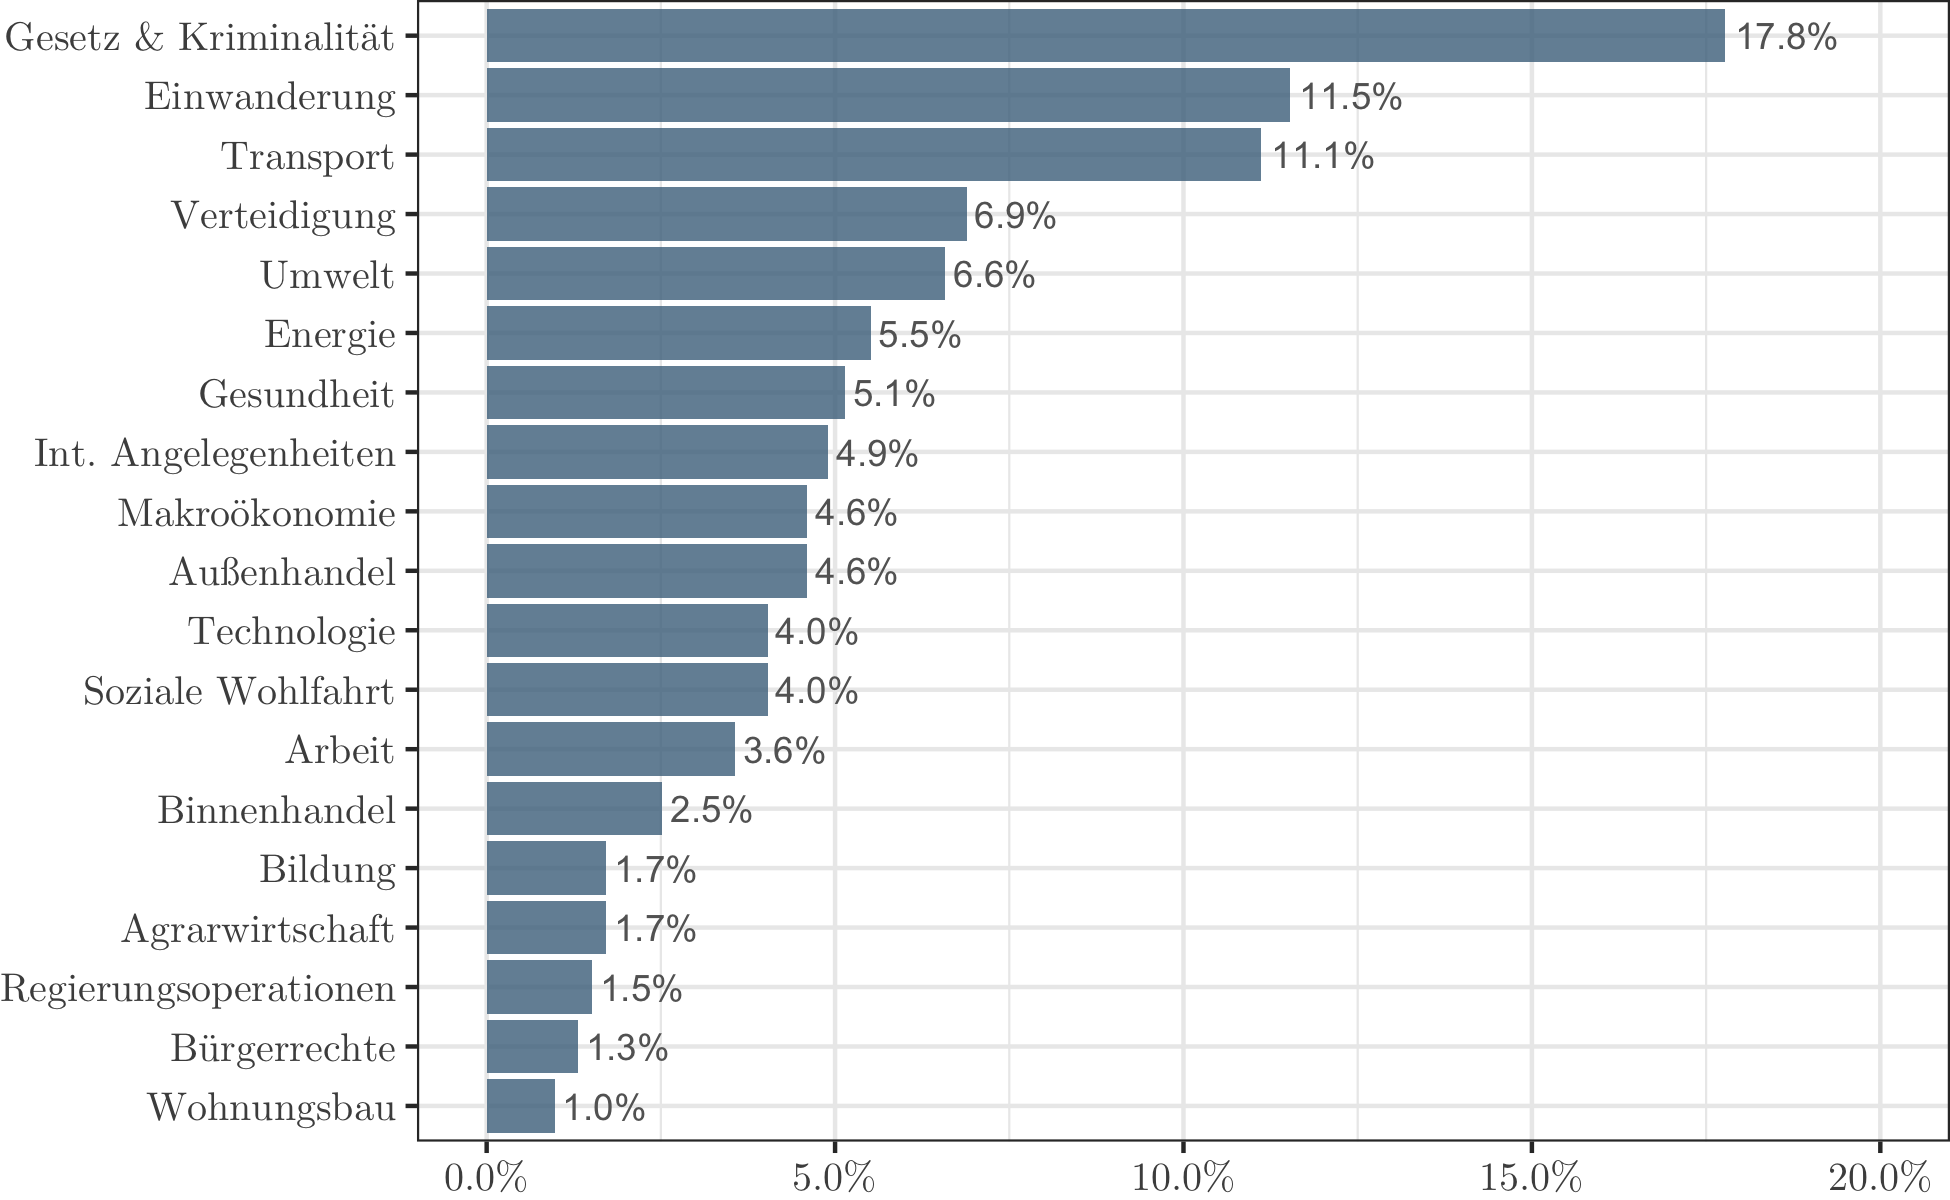
\includegraphics[width=\textwidth]{images/themen_gesamt_manual_matching_test.png}
    \caption*{\scriptsize }
\end{figure}

Dabei wird ersichtlich, dass die Themen \emph{Gesetz \& Kriminalität},
\emph{Einwanderung} und \emph{Transport} jeweils einen Anteil von
mindestens 10\% der klassifizierten Themen aufweisen. Gleichzeitig
liegen Themen wie \emph{Wohnungsbau}, \emph{Bürgerrechte} und
\emph{Regierungsoperationen} vor, welche jeweils nur einen Anteil von
0,6 bis gut 2,1 Prozent ausmachen.

Anteil aller bla bla Test Datensatz blub

\begin{table}[ht]
\centering
\caption{Richtig kategorisierte Anfragen und Anteil der Klassifikationen}
\begin{tabular}{lllllllll}
$p$   & \multicolumn{2}{c}{$RF_{200}$} & \multicolumn{2}{c}{$RF_{500}$} & \multicolumn{2}{c}{$RF_{1500}$} & \multicolumn{2}{c}{$SVM_{C = 10}$} \\
   \hline
    & Richtig      & Anteil      & Richtig      & Anteil      & Richtig       & Anteil      & Richtig     & Anteil    \\
   \hline
 0.3 &   83,89    &    74,83  &    84,96    &   73,89   &   85,08     &   72,69   &  80,91   &   76,45  \\
 0.4 &   90,07    &    58,00  &    89,47    &   58,50   &   90,42     &   57,29   &  85,54   &   64,79  \\
 0.5 &   94,21    &    41,63  &    93,08    &   42,57   &   93,13     &   42,84   &  88,30   &   52,61  \\
 0.6 &   97,73    &    29,45  &    97,33    &   30,12   &   96,77     &   29,05   &  89,02   &   46,32  \\
 0.7 &   100      &    19,54  &    99,33    &   19,95   &   100       &   19,14   &  91,75   &   40,56 \\
 0.8 &   100      &    13,12  &    100      &   13,38   &   100       &   12,58   &  92,68   &   32,93  \\
 0.9 &   100      &     9,77  &    100      &    9,91   &   100       &    9,91   &  95,43   &   23,43  \\
 \hline
mean   & 95,40    &   34,56   &    94,73    &   36,37   &   95,06     &   34,79   &  89,09   &   48,16  \\
  \hline
\end{tabular}
\caption*{\scriptsize Anmerkung: Angaben in Prozent; $p$ stellt den Cutt Off für die Klassenwahrscheinlichkeit dar}
\end{table}

Klassenwahrscheinlichkeiten im einzelnen\ldots{}blub\ldots{}aber Test
blüb

\begin{figure}[!h]
    \caption{Klassenwahrscheinlichkeiten (Testklassifikation)}
    \label{probs_real}
    \centering
    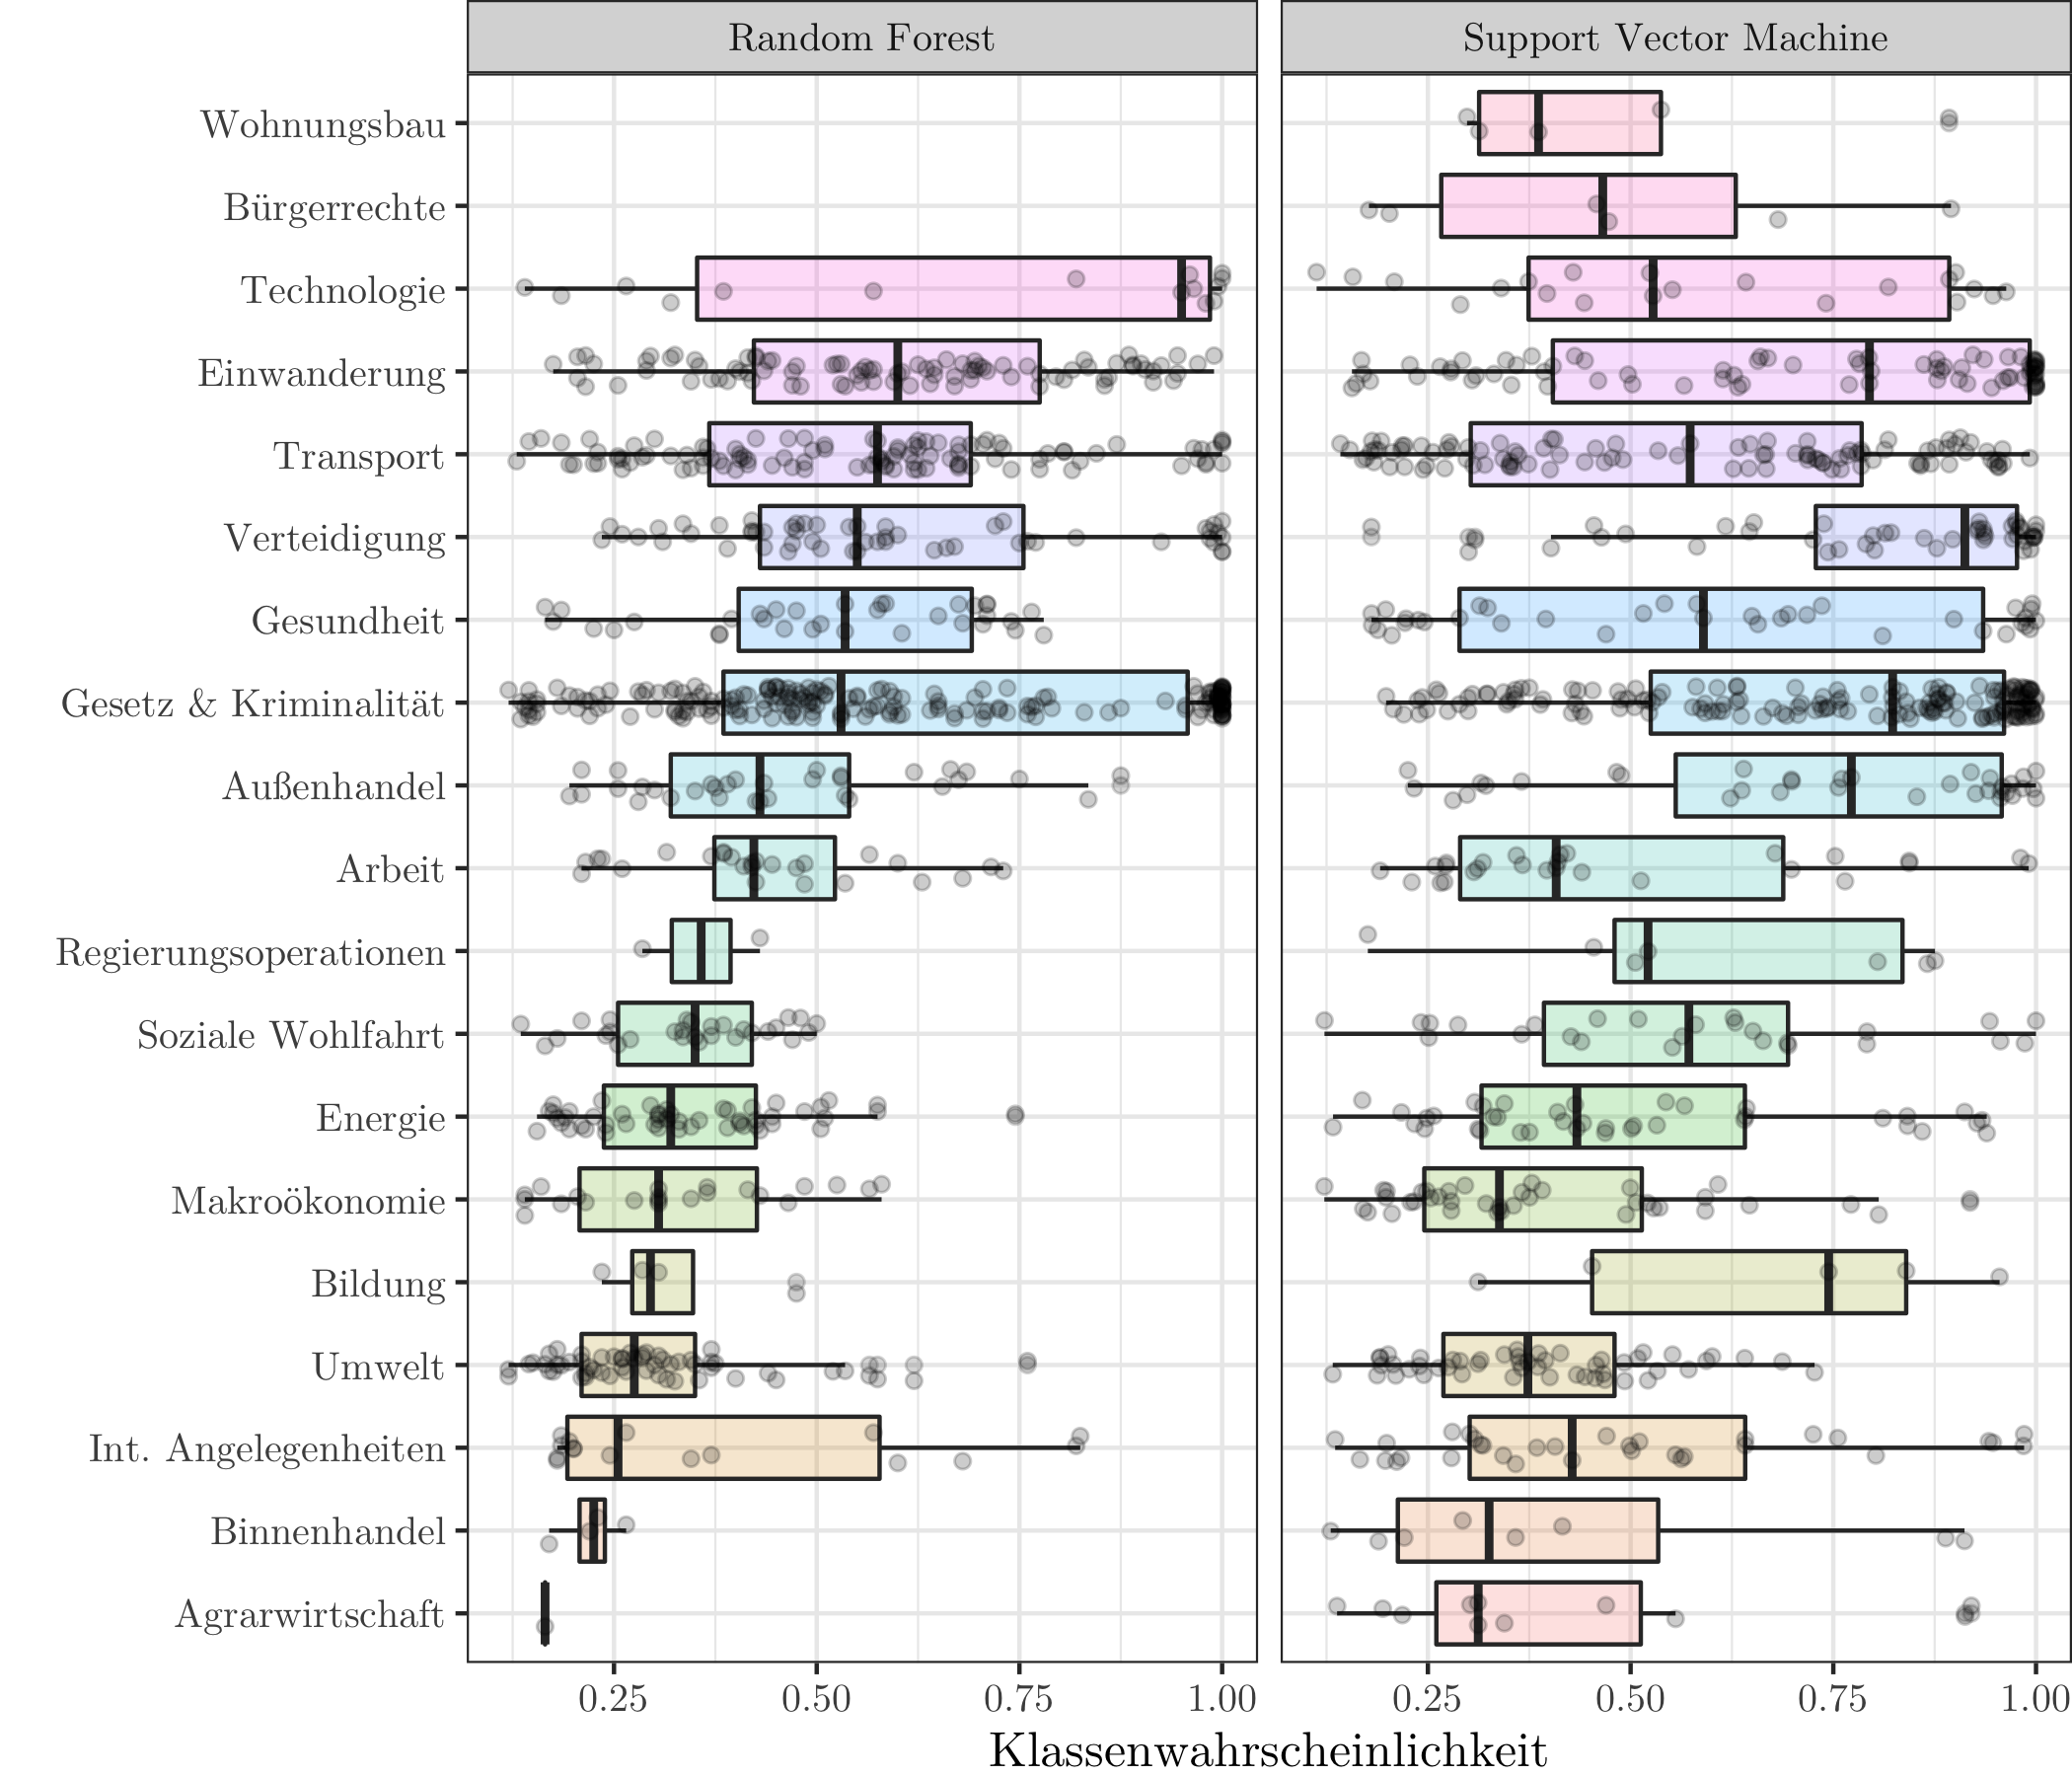
\includegraphics[width=\textwidth]{images/rf_svm_prob_boxplot_2.png}
    \caption*{\scriptsize }
\end{figure}

Klassenwahrscheinlichkeiten für vollständige Klassifikation (Apendix, da
kaum Unterschiede mit Testklassifikation\ldots{})

\begin{figure}[!h]
    \caption{Klassenwahrscheinlichkeiten (vollständige Klassifikation)}
    \label{probs_real}
    \centering
    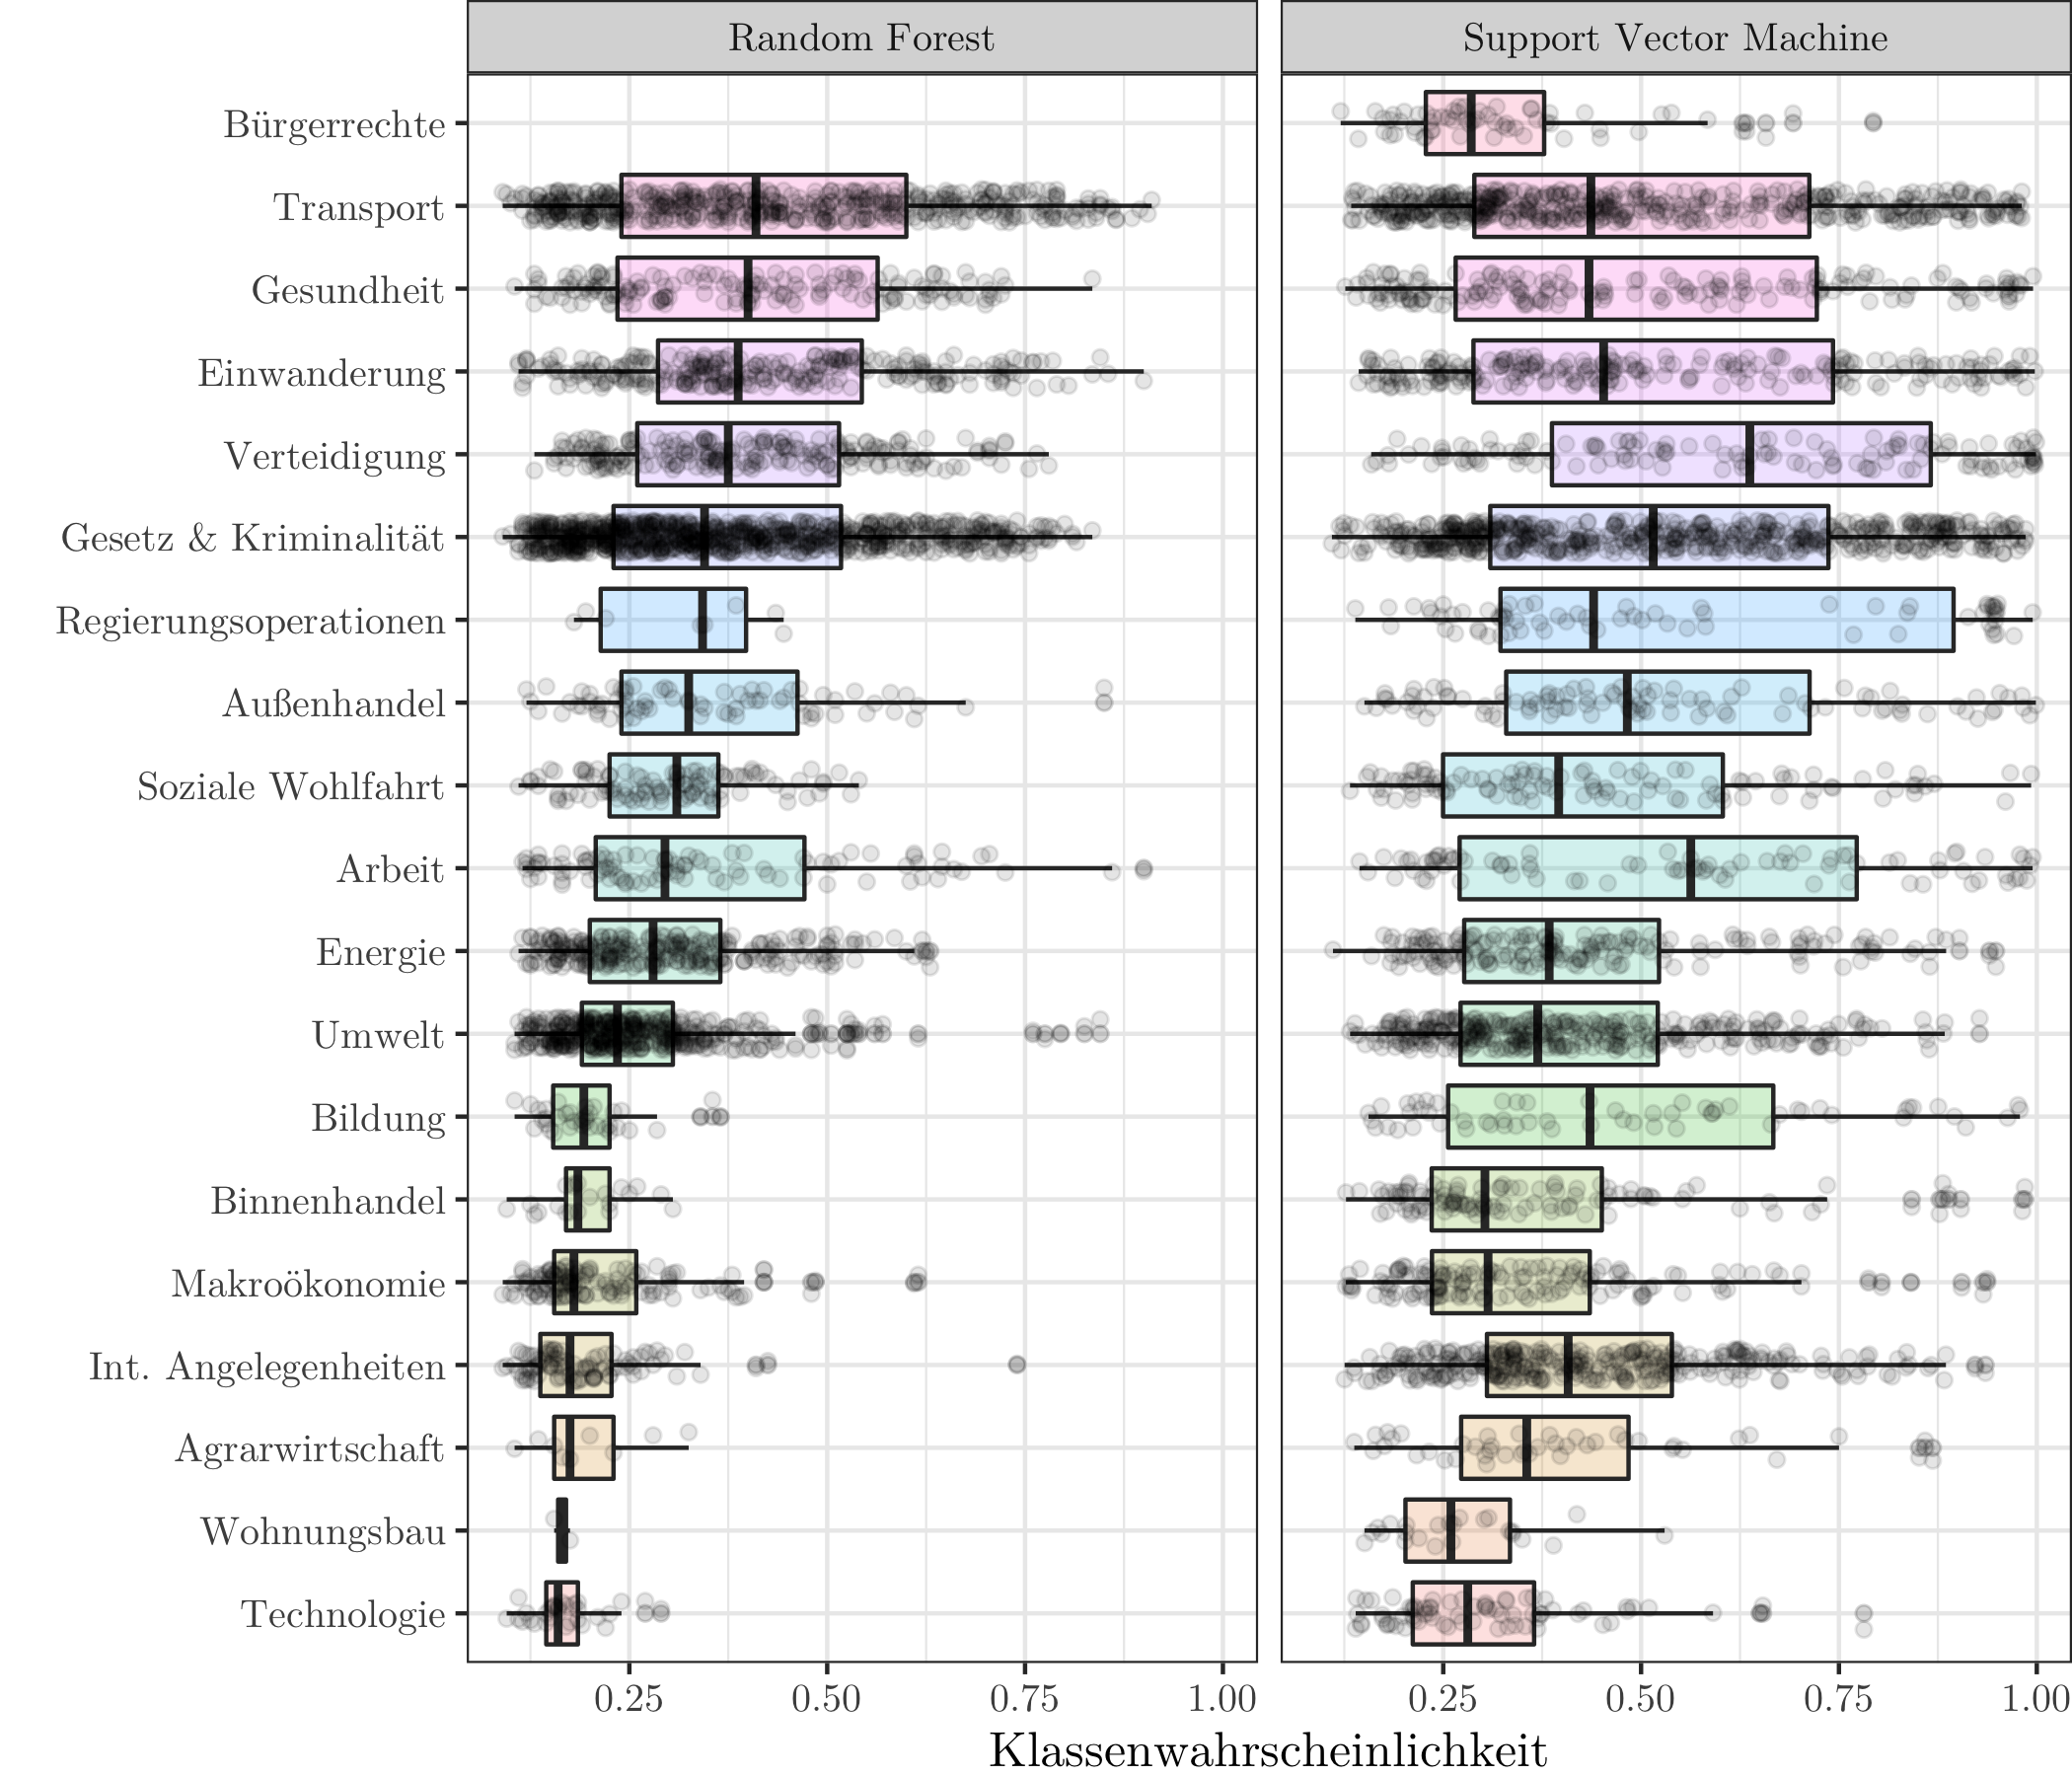
\includegraphics[width=\textwidth]{images/prob_boxplot_real_mod_2.png}
    \caption*{\scriptsize }
\end{figure}

\subsection{Deskriptive Analyse}\label{deskriptive-analyse}

Darstellung der Anfragen nach Partei

\begin{figure}[!h]
    \caption{Anzahl gestellter Anfragen nach Partei}
    \label{anfragen_count}
    \centering
    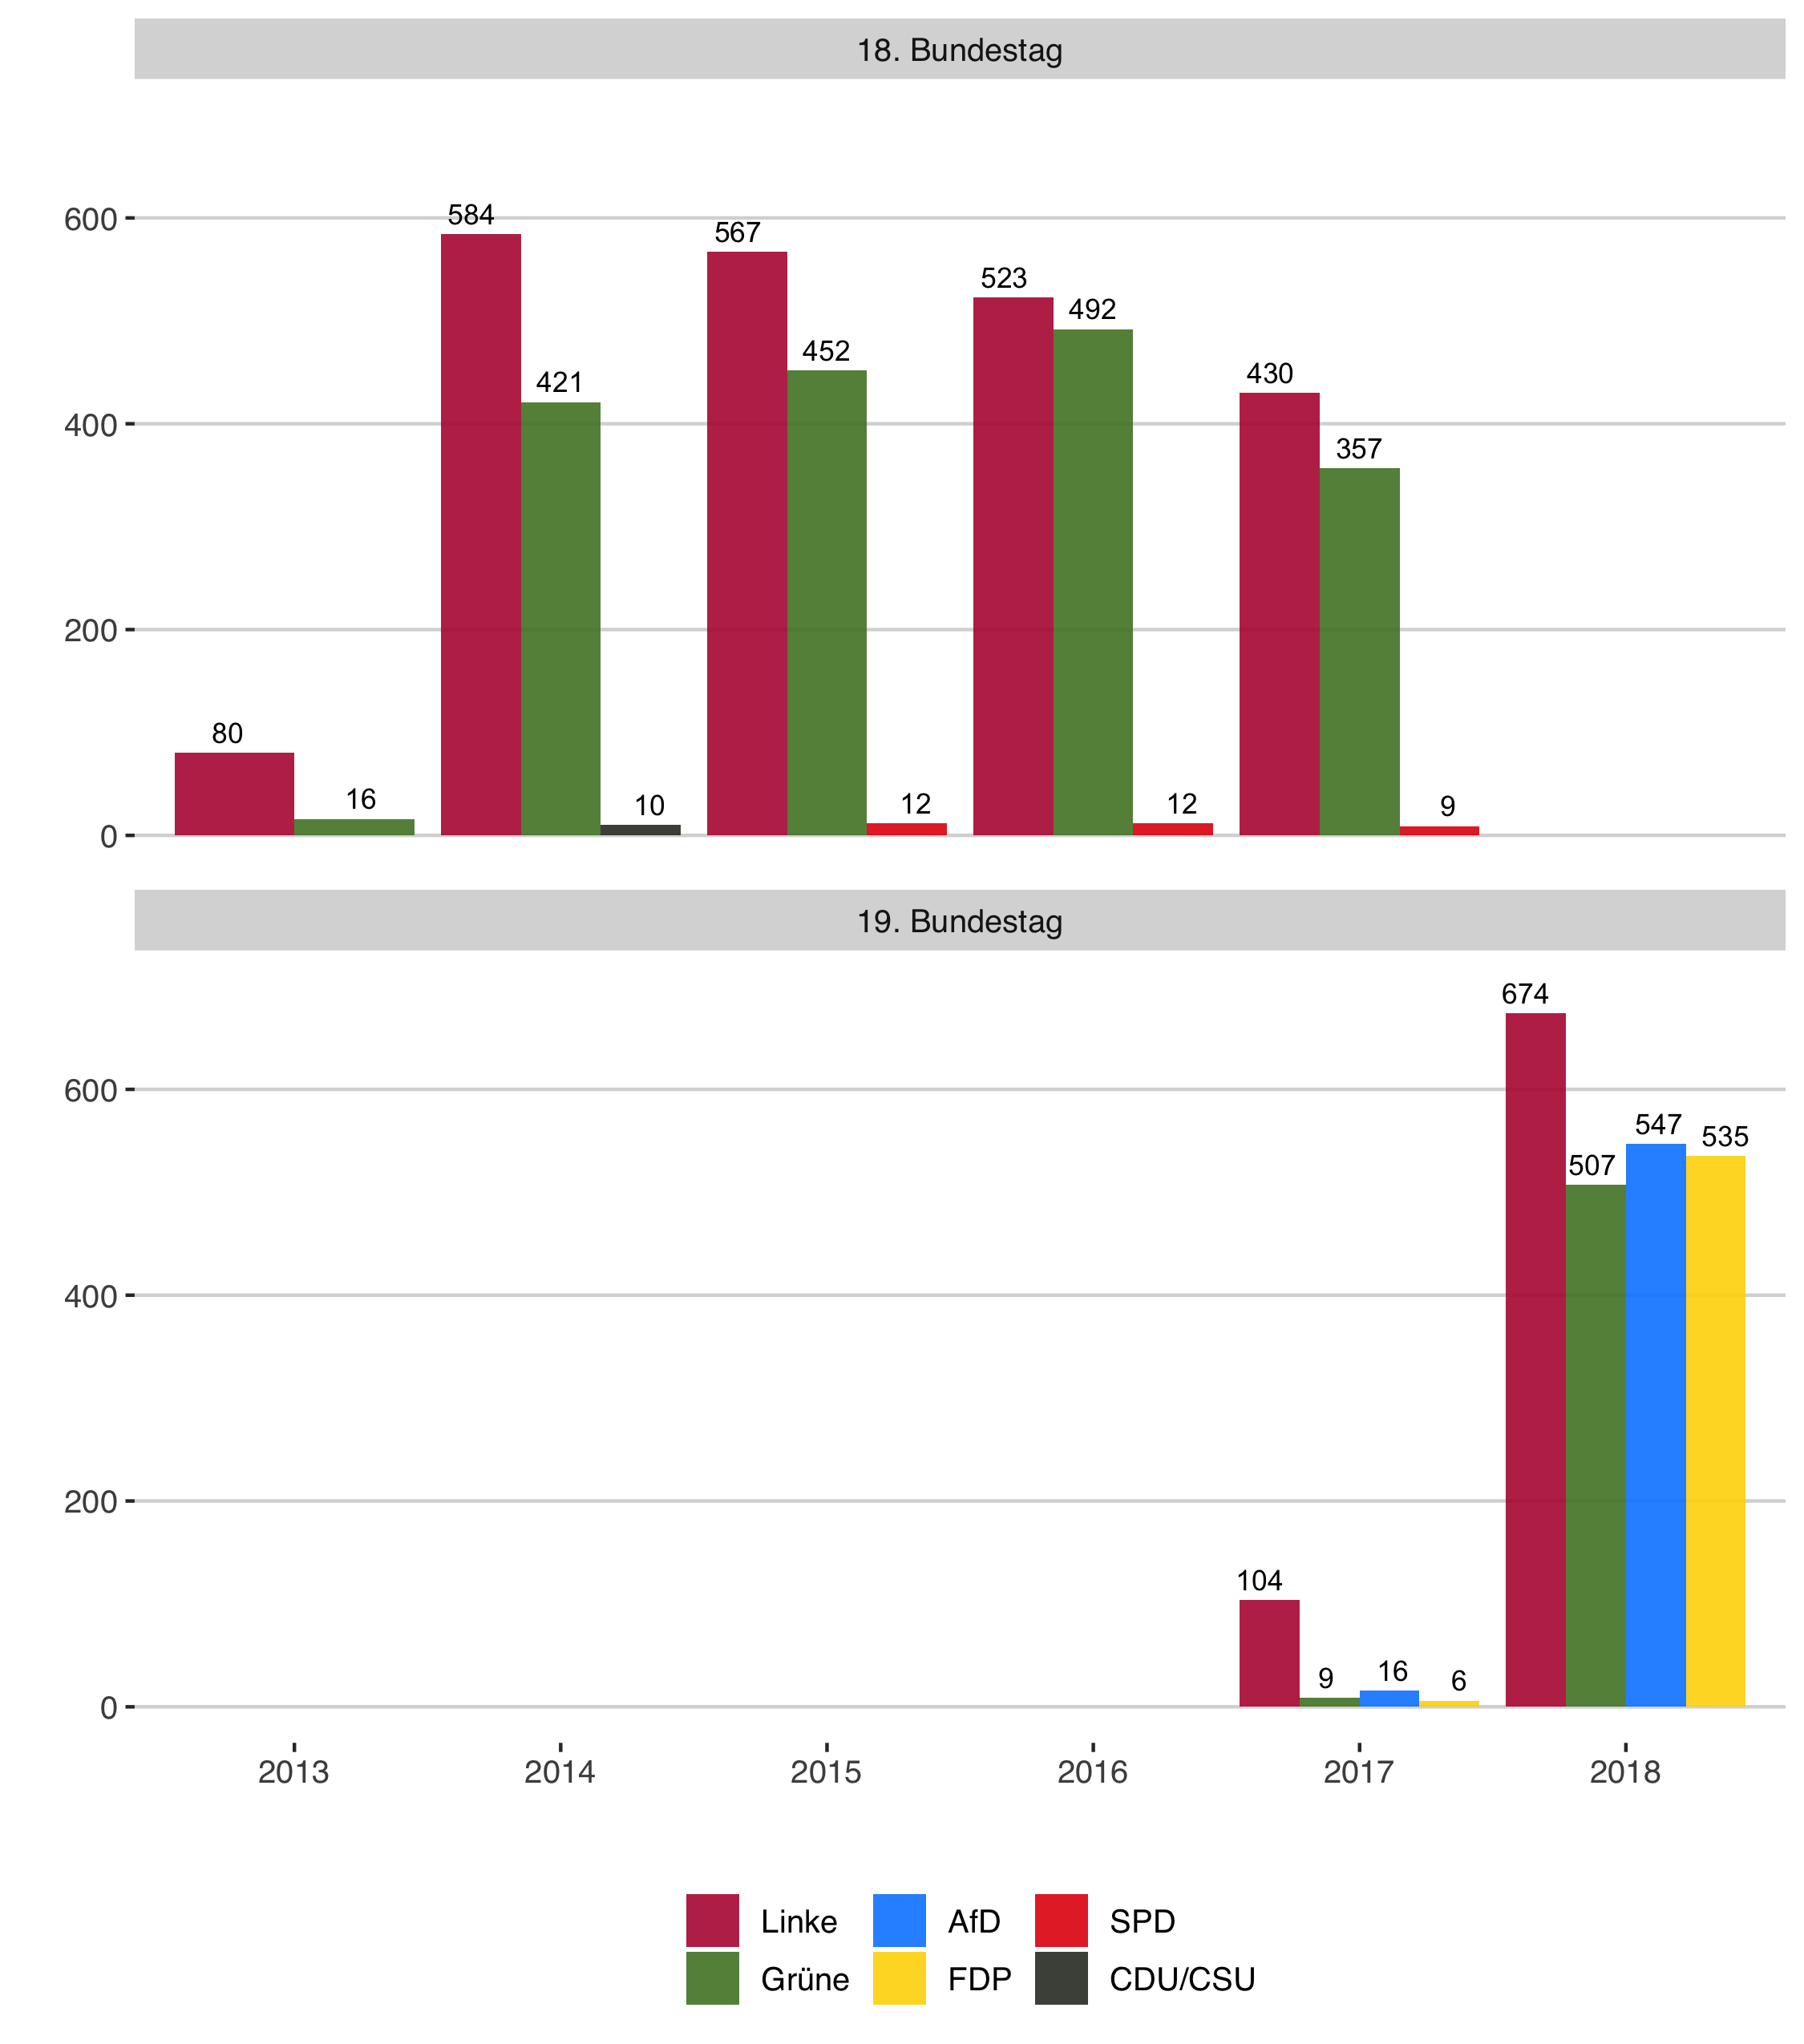
\includegraphics[width=\textwidth]{images/AnfragenPartei_18_19_complete.png}
    \caption*{\scriptsize Anmerkung: Anzahl der kleinen Anfragen nach Jahr und Legislaturperiode}
\end{figure}

\subsection{Sentiment Analyse}\label{sentiment-analyse}


\end{document}
